\section{Controller design}
In this section the controller architecture is discussed, initially the entire architecture
is described then each controller is extensively analyzed.
The main idea is develop a cascade control architecture (see Figure \ref{fig:control_architecuture}).
The inner allows is used to tracking the
Zero Momentum point trajectory while the outer loop is necessary to stabilize the
CP unstable dynamics (\ref{eq:cp_dynamics}).
\begin{figure}[!ht]
  \centering
  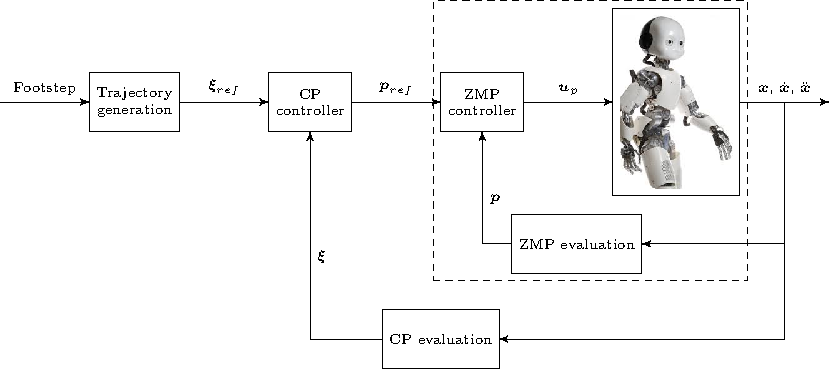
\includegraphics[scale=1.0]{control_architecture}
  \caption{Controller architecture. \label{fig:control_architecuture}}
\end{figure}
It is important to underline that in the controller synthesis the following assumption holds:
\begin{itemize}
\item[-] the position, velocity and acceleration of the CoM of the entire robot can be measured or,
  in general, derived;
\item[-] the jerk of the CoM $\dddot{\vec{x}}$ is the controlled input.
\end{itemize}

\subsection{Capture Point Controller}
Several version of capture point controller was proposed in these last years,
for example Englsberger proposed a linear feedback controller \cite{Englsberger2011}
while Krause a MPC approach \cite{Krause2012}.
Both of these architecture use the ZMP as the controlled variable and in order to respect the
constraints on the ZMP (see the principle \ref{principle:zmp}) in the linear controller approach
a projection inside the support polygon was proposed; while in the MPC approach the ZMP constraint
was incorporated in the MPC framework.
In the following dissertation the MPC approach is proposed.
\par
The aim of this approach is stabilizing only the unstable part of the CP dynamics
(\ref{eq:cp_dynamics}). The following dynamic equation is used as the prediction model
\begin{equation}
  \label{eq:cp_dynamics_vettorial}
  \dot{\vec{\xi}} = \omega(\vec{\xi} - \vec{p})
\end{equation}
where $\vec{\xi}$ is the vector that contains the $x$ and $y$ coordinates of the capture point,
while $\vec{p}$, the control input, contains the  $x$ and $y$ coordinates of the ZMP.
In the following a discrete time implementation with a piecewise constant control inputs.
The equation (\ref{eq:cp_dynamics_vettorial}) can be discretized
\[
\vec{\xi}_{k+1} = A \vec{\xi}_{k} + B \vec{p}_{k} =
\begin{bmatrix}
  e^{\omega T} & 0 \\
  0 & e^{\omega T} \\
\end{bmatrix}
\vec{\xi}_{k} +
\begin{bmatrix}
  1-e^{\omega T} \\
  1-e^{\omega T}
\end{bmatrix}
\vec{p}_{k} 
\]
where $T$ is the sampling time. In order to reduce the number of variable in the MPC problem the
``single shooting'' approach is used. The main idea is to keep only $\vec{\xi}_k$ and the vector
input $\vec{P}$ as variables and the states $\vec{\xi}_{k + 1}, \dots, \vec{\xi}_{k + N}$ are eliminated recursively.
Thus, the predicted capture point for the next $N$ states can be summarized as follows
\[
\vec{\Xi} = F_{\xi} \vec{\xi}_k + F_{p} \vec{P}
\]
where
\[
\vec{\Xi} =
\begin{bmatrix}
  \vec{\xi}_{k+1}\\
  \vdots\\
  \vec{\xi}_{k+N}
\end{bmatrix} \quad
\vec{P} =
\begin{bmatrix}
  \vec{p}_{k}\\
  \vdots\\
  \vec{p}_{k+N-1}
\end{bmatrix}
\]
and
\[
F_{\xi} =
\begin{bmatrix}
  A\\
  \vdots\\
  A^N
\end{bmatrix} \quad
F_p =
\begin{bmatrix}
  B & \hdots & 0\\
  \vdots &\ddots & \vdots\\
  A^{N-1} B & \hdots & B
\end{bmatrix}
\]
The control objective is the tracking the reference CP trajectory $\vec{\xi}_{ref}$ while the ZMP
position satisfies the well known constraint.
Thus the following objective function can be defined
\[
J_k = \frac{1}{2} \left\{  (\vec{\Xi}_{ref} - \vec{\Xi})\transpose Q (\vec{\Xi}_{ref} - \vec{\Xi}) +
(\Theta \vec{P} - \vec{e}_1 \vec{p}_{k-1}) \transpose R (\Theta \vec{P} - \vec{e}_1 \vec{p}_{k-1}) \right\}
\]
where $Q$ and $R$ are symmetric and positive definite matrices and $(\Theta \vec{P} - \vec{e}_1 \vec{p}_{k-1})$ is the rate of change of the controlled input. More specifically the matrix $\Theta$ is
defined as follow
\[
\Theta =
\begin{bmatrix}
  I & 0 & \hdots & 0 \\
  I & -I & \hdots & 0 \\
  \vdots & \vdots & \ddots & \vdots \\
  0 & 0 & \hdots & -I
\end{bmatrix}
\]
In order to embedded the ZMP constraint in the MPC framework the position the following inequality
must hold
\[
\vec{f}_{min} \le {}^f R_g(\alpha_k) ({}^g \vec{p}_k - {}^ g \vec{r}_k) \le \vec{f}_{max}
\]
where ${}^f R_g(\alpha_k)$ is the rotation matrix between the reference frame attached to the
reference foot and the global inertial frame (see Figure \ref{fig:control_architecuture});
$\vec{r}_k$ and $\alpha_k$ are respectively the footstep position and the orientation provided
by the footstep planning algorithm. Finally $\vec{f}_{min}$ and $\vec{f}_{max}$ are the minimum and
maximum values determined by rectangular envelope (draw in red in the figure
\ref{fig:control_architecuture}).
\begin{figure}[!ht]
  \centering
  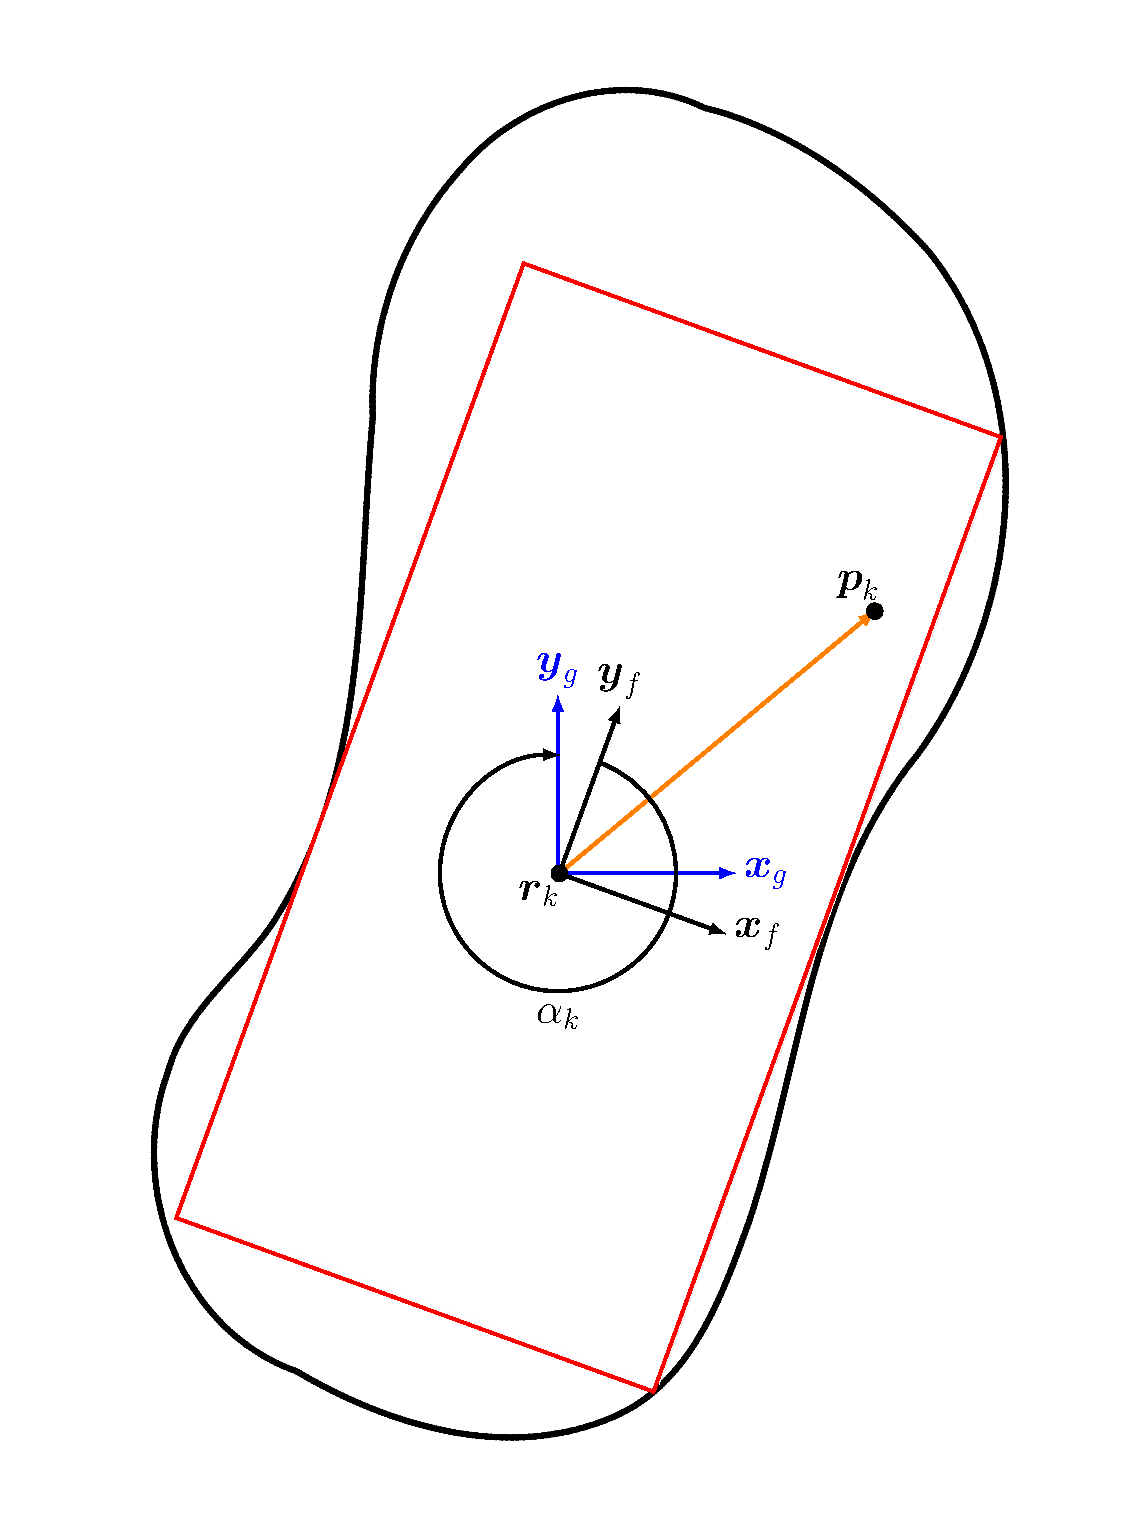
\includegraphics[scale=.4]{foot_support_polygon}
  \caption{Controller architecture. \label{fig:control_architecuture}}
\end{figure}
\par
In summary the following optimization problem has to be solved is
\[
\begin{split}
  \min_{\vec{P}, \vec{\xi}_k} &  \quad \left[  \frac{1}{2}\left\{ (\vec{\Xi}_{ref} - \vec{\Xi})\transpose Q (\vec{\Xi}_{ref} - \vec{\Xi}) + (\Theta \vec{P} - \vec{e}_1 \vec{p}_{k-1}) \transpose R (\Theta \vec{P} - \vec{e}_1 \vec{p}_{k-1}) \right\} \right]\\
  \text{s.t.} & \quad \quad \quad  F_{\xi} \vec{\xi}_k + F_{p} \vec{P}  - \vec{\Xi} = \vec{0}\\
  & \quad \quad \quad  \vec{f}_{min} \le {}^f R_g(\alpha_k) ({}^g \vec{p}_k - {}^ g \vec{r}_k) \le \vec{f}_{max}
\end{split}
\]
\subsection{Zero Momentum Point Controller}
In this section the inner zero momentum point controller is analyzed. This approach is based on the
Kajita work \cite{Kajita2003}.
Using the well known ZMP equations and the the fact that the two equation are decoupled
\[
\begin{split}
  p_y = y - \frac{z_c}{g} \ddot{y}\\
  p_x = x - \frac{z_c}{g} \ddot{y}
\end{split}
\]
the following dynamic system can be defined
\begin{equation}
  \label{eq:zmp_mpc}
  \begin{bmatrix}
    \dot{x} \\
    \ddot{x} \\
    \dddot{x}
  \end{bmatrix} =
  \begin{bmatrix}
    0 & 1 & 0 \\
    0 & 0 & 1 \\
    0 & 0 & 0
  \end{bmatrix}
  \begin{bmatrix}
    x \\
    \dot{x} \\
    \ddot{x}
  \end{bmatrix}
  +
  \begin{bmatrix}
    0 \\
    0 \\
    1 
  \end{bmatrix}
  u_x
\end{equation}
\begin{equation}
  \label{eq:zmp_mpc_y}
  p_x =
  \begin{bmatrix}
    1 & 0 & -\frac{z_c}{g}
  \end{bmatrix}
  \begin{bmatrix}
    x \\
    \dot{x} \\
    \ddot{x}
  \end{bmatrix}
\end{equation}
the same system can be obtained for the $y$-coordinate.
\par
An MPC controller can be synthesize using the equations \ref{eq:zmp_mpc} and \ref{eq:zmp_mpc_y}.
First of all the ZMP dynamic equation must be discretized with a fixed sampling time $T$.
\[
\begin{split}
  &\vec{x}_{k + 1} = A \vec{x}_k + B u_k\\
  &p_k = C \vec{x}_{k}
\end{split}
\]
where
\[
A = \begin{bmatrix}
  1 & T & \frac{T^2}{2}\\
  0 & 1 & T \\
  0 & 0 & 1
\end{bmatrix} \quad
B = \begin{bmatrix}
  \frac{T^3}{6}\\
  \frac{T^2}{2}\\
  T
\end{bmatrix}\quad
C =  \begin{bmatrix}
    1 & 0 & -\frac{z_c}{g}
  \end{bmatrix}
\]
The same approach shown in the previous section can be followed in order to formalize the optimal
problem.
Only $\vec{x}_k$ and the vector
input $\vec{U}$ as variables and the states $\vec{x}_{k + 1}, \dots, \vec{x}_{k + N}$ are eliminated recursively.
Thus, the predicted dynamic system for the next $N$ states can be summarized as follows
\[
\vec{X} = F_{x} \vec{x}_k + F_{u} \vec{U}
\]
where
\[
\vec{X} =
\begin{bmatrix}
  \vec{x}_{k+1}\\
  \vdots\\
  \vec{x}_{k+N}
\end{bmatrix} \quad
\vec{U} =
\begin{bmatrix}
  \vec{u}_{k}\\
  \vdots\\
  \vec{u}_{k+N-1}
\end{bmatrix}
\]
and
\[
F_{x} =
\begin{bmatrix}
  A\\
  \vdots\\
  A^N
\end{bmatrix} \quad
F_u =
\begin{bmatrix}
  B & \hdots & 0\\
  \vdots &\ddots & \vdots\\
  A^{N-1} B & \hdots & B
\end{bmatrix}
\]
While the output equation becomes
\[
\vec{P} = H_{x} \vec{x}_k + H_{u} \vec{U}
\]
where
\[
\vec{P} =
\begin{bmatrix}
  p_{k}\\
  \vdots\\
  p_{k+N}
\end{bmatrix}
\]
and
\[
H_{x} =
\begin{bmatrix}
  C \\
  CA \\
  \vdots\\
  C A^{N}
\end{bmatrix} \quad
H_u =
\begin{bmatrix}
  0 & 0 & \hdots & 0\\
  CB & 0 & \hdots &  0 \\
  CBA & CB & \hdots &  0 \\
  \vdots & \vdots & \ddots & \vdots \\ 
    CBA^{N-1} & CBA^{N-2} & \hdots &  C 
\end{bmatrix}
\]
The following objective function is chosen
\[
\frac{1}{2} \left\{ (\vec{P}_{ref} - \vec{P})\transpose Q_p (\vec{P}_{ref} - \vec{P}) +
\vec{\Delta U} \transpose R \vec{\Delta U} + 
\vec{\Delta X} \transpose Q_x \vec{\Delta x} \right\}
\]
where
\[
\vec{P} =
\begin{bmatrix}
  p_k \\
  p_{k + 1} \\
  \vdots \\
  p_{k + N -1}
\end{bmatrix} \quad
\vec{\Delta X} =
\begin{bmatrix}
  \vec{x}_k - \vec{x}_{k+1} \\
  \vec{x}_{k + 1} - \vec{x}_{k + 2} \\
  \vdots \\
  \vec{x}_{k + N - 1} - \vec{x}_{k + N}
\end{bmatrix} \quad
\vec{\Delta U} =
\begin{bmatrix}
  u_k - u_{k+1} \\
  u_{k + 1} - u_{k + 2} \\
  \vdots \\
  u_{k + N - 2} - u_{k + N - 1}
\end{bmatrix}
\]
while the matrix $Q_p$, $Q_x$ and $R$ are positive and non-negative definite matrix.
Last but not least the reference input $\vec{P}_{ref}$ is the output of the capture point controller
developed in the previus section.
\par
The MPC problem can be summarized as a Quadratic Programming Problem:
\[
\begin{split}
  \min_{\vec{U}, \vec{x}_k} &  \quad \left[\frac{1}{2} \left\{ (\vec{P}_{ref} - \vec{P})\transpose Q_p (\vec{P}_{ref} - \vec{P}) +
\vec{\Delta U} \transpose R \vec{\Delta U} + 
\vec{\Delta X} \transpose Q_x \vec{\Delta x} \right\} \right ]\\
  \text{s.t.} & \quad \quad \quad  F_{x} \vec{x}_k + F_{u} \vec{U} - \vec{X} = \vec{0}\\
  & \quad \quad \quad  H_{x} \vec{x}_k + H_{u} \vec{U} - \vec{P} = \vec{0}
\end{split}
\]
